% ============================================================================
% IGVC 2026 Design Report
% Cal Poly Pomona Autonomous Vehicle Lab
%
% Page budget (~15 pages total):
%   - Title + TOC:                       ~2 pages
%   - Sections 1-3 (team / arch / inn):  ~3 pages
%   - Mechanical placeholder (PDF):      ~2-3 pages (insert your subteam PDF)
%   - Electrical placeholder (PDF):      ~2-3 pages (insert your subteam PDF)
%   - Software (Sec 6) + AutoNav (Sec 9): ~5-6 pages
%   - Cyber + Analysis + Performance:    ~2 pages
% ============================================================================
\documentclass[11pt, letterpaper]{article}

\usepackage[margin=1in]{geometry}
\usepackage{graphicx}
\usepackage{booktabs}
\usepackage{tabularx}
\usepackage{amsmath}
\usepackage{amssymb}
\usepackage{hyperref}
\usepackage{xcolor}
\usepackage{float}
\usepackage{enumitem}
\usepackage{caption}
\usepackage{tikz}
\usepackage{pdfpages}
\usepackage{fancyhdr}
\usepackage{titlesec}
\usepackage{array}
\usepackage{multirow}
\usepackage[T1]{fontenc}
\usepackage[nottoc]{tocbibind}

\usetikzlibrary{shapes.geometric, arrows.meta, positioning, fit, calc, backgrounds}

% ---- Colors ----
\definecolor{cppgreen}{RGB}{30, 90, 50}
\definecolor{codeblue}{RGB}{0, 80, 160}

% ---- Hyperref ----
\hypersetup{colorlinks=true, linkcolor=cppgreen, citecolor=cppgreen, urlcolor=codeblue}

% ---- Headers / Footers ----
\pagestyle{fancy}
\fancyhf{}
\fancyhead[L]{\small Cal Poly Pomona Autonomous Vehicle Lab}
\fancyhead[R]{\small IGVC 2026 Design Report}
\fancyfoot[C]{\thepage}
\renewcommand{\headrulewidth}{0.4pt}

% ---- Section formatting (compact) ----
\titleformat{\section}{\large\bfseries\color{cppgreen}}{\thesection.}{0.5em}{}
\titleformat{\subsection}{\normalsize\bfseries}{\thesubsection}{0.5em}{}
\titlespacing*{\section}{0pt}{1.2ex}{0.6ex}
\titlespacing*{\subsection}{0pt}{0.8ex}{0.3ex}

% ---- Macros ----
\newcommand{\placeholder}[1]{\textcolor{red}{\textbf{[#1]}}}
\newcommand{\robotname}{PLACEHOLDER\_ROBOT\_NAME}
\newcommand{\teamname}{Cal Poly Pomona Autonomous Vehicle Lab}
\newcommand{\university}{California State Polytechnic University, Pomona}

% Tighter lists
\setlist[itemize]{noitemsep, topsep=2pt, leftmargin=*}
\setlist[enumerate]{noitemsep, topsep=2pt, leftmargin=*}

\begin{document}

% ============================================================================
% TITLE PAGE
% ============================================================================
\begin{titlepage}
    \centering
    \vspace*{0.8cm}

    {\Large \university \par}
    \vspace{0.25cm}
    {\Large \teamname \par}
    \vspace{0.25cm}
    {\LARGE\bfseries IGVC 2026 Design Report \par}
    \vspace{0.25cm}
    {\Large \robotname \par}

    \vspace{0.7cm}
    \placeholder{Insert robot photo: figures/robot\_photo.jpg}
    % \includegraphics[width=0.55\textwidth]{figures/robot_photo.jpg}

    \vspace{0.5cm}

    \textit{I hereby certify that the development of the vehicle, \robotname{}, as described in this report,\\
    is equivalent to the work involved in a senior design course.}

    \vspace{0.25cm}
    Submitted \placeholder{Month Day}, 2026

    \vspace{0.8cm}

    \begin{tabular}{l l l}
        \toprule
        \textbf{Software} & \textbf{Mechanical} & \textbf{Electrical} \\
        \midrule
        \placeholder{Parsa Ghasemi (Lead)} & \placeholder{Name (Lead)} & \placeholder{Name (Lead)} \\
        \placeholder{Caleb Hylkema} & \placeholder{Name} & \placeholder{Name} \\
        \placeholder{Name} & \placeholder{Name} & \placeholder{Name} \\
        \placeholder{Name} & \placeholder{Name} & \placeholder{Name} \\
        \bottomrule
    \end{tabular}

    \vspace{0.8cm}

    \textbf{Faculty Advisor:} \placeholder{Dr.~Advisor Name, Department of Electrical and Computer Engineering}

    \vspace{0.25cm}
    Faculty Signature: \rule{6cm}{0.4pt} \quad Date: \rule{2cm}{0.4pt}

\end{titlepage}

% ============================================================================
% TABLE OF CONTENTS
% ============================================================================
\tableofcontents
\thispagestyle{fancy}
\newpage

% ============================================================================
% 1. DESIGN PROCESS, TEAM, ORGANIZATION
% ============================================================================
\section{Design Process, Team Identification, and Organization}

\subsection{Introduction}

The \teamname{} (AVL) at \university{} presents \robotname{}, our entry for the
2026 Intelligent Ground Vehicle Competition (IGVC) in both the AutoNav and Self-Drive
challenges. AVL is an undergraduate research lab within the College of Engineering focused
on autonomy, embedded systems, and ground-vehicle perception. The IGVC subteam consists of
\placeholder{N} students organized across three disciplines: software, mechanical, and
electrical, advised by \placeholder{Dr.~Advisor Name}.

\robotname{} is a fully autonomous differential-drive tracked vehicle built on the AVL's
drive-by-wire research platform (AndyMark Raptor chassis). The robot fuses a Velodyne VLP-16
3D LiDAR, three Stereolabs ZED~X stereo cameras (front/left/right), and an Xsens MTi-680G
IMU+GNSS for perception and localization, with all autonomy software running on an NVIDIA
Jetson Orin under ROS~2 Humble.

\subsection{Team Organization}

The IGVC team is led by a project captain and divided into three subteams reporting to the
captain. The software subteam owns perception, localization, planning, control, and
firmware. The mechanical subteam owns chassis, drivetrain, sensor mounting, and
weatherproofing. The electrical subteam owns power distribution, wiring, and the
safety interlock circuit. Weekly all-hands meetings keep subteams synchronized; biweekly
integration days exercise the full vehicle on the test course.

\subsection{Design Process}

The team follows an iterative cycle of \textit{research $\rightarrow$ design
$\rightarrow$ prototype $\rightarrow$ test}, executed in four phases over the academic
year:

\begin{enumerate}
    \item \textbf{Requirements and rules analysis.} Re-read of the IGVC 2026 rulebook, review of recent winning design reports (notably Sooner Robotics 2025 and Ville Robotics 2024), and definition of system-level requirements for chassis, sensor suite, compute, and software stack.
    \item \textbf{Subsystem development.} Each subteam develops its components independently --- mechanical CAD, electrical schematics, ROS~2 packages, and Teensy firmware.
    \item \textbf{Integration.} Subsystems are integrated incrementally: firmware on the bench (Phases 1--7 of motor characterization), then attached to the actuator node, then sensor fusion, then full Nav2 stack.
    \item \textbf{Field testing.} Iterative outdoor testing on the \placeholder{CPP test area}, with data-driven tuning of HSV perception thresholds, EKF covariances, costmap parameters, and MPPI critic weights.
\end{enumerate}

% ============================================================================
% 2. SYSTEM ARCHITECTURE
% ============================================================================
\section{System Architecture}

\robotname{} is organized into five functional layers: \textbf{sensing}, \textbf{perception},
\textbf{localization}, \textbf{navigation}, and \textbf{actuation}. All software runs on the
Jetson Orin under ROS~2 Humble with CycloneDDS middleware. A Teensy~4.1 microcontroller bridges
the Jetson (USB serial) to two REV SparkMAX motor controllers (CAN bus at 1~Mbit/s).
Figure~\ref{fig:system_arch} shows the high-level dataflow.

\begin{figure}[H]
    \centering
    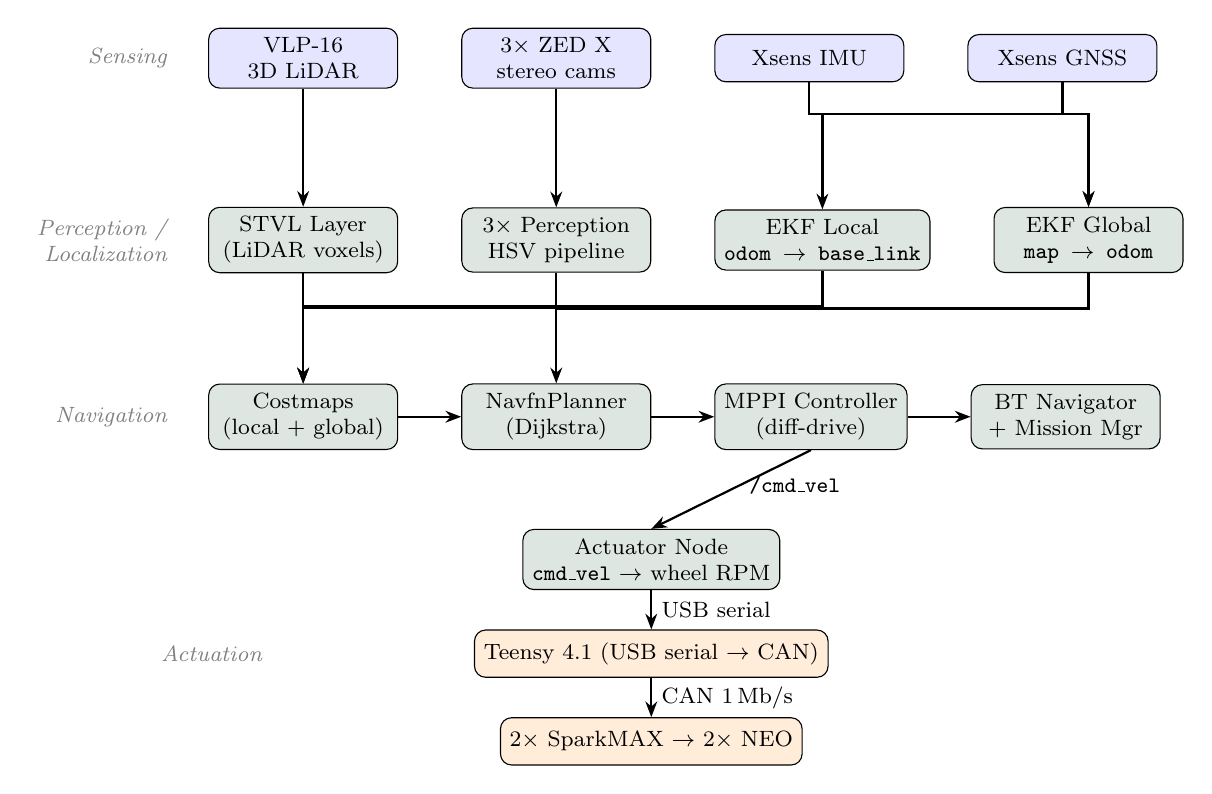
\begin{tikzpicture}[
        font=\footnotesize,
        sensor/.style={draw, rounded corners, fill=blue!10, minimum width=2.4cm, minimum height=0.6cm, align=center},
        block/.style={draw, rounded corners, fill=cppgreen!15, minimum width=2.4cm, minimum height=0.6cm, align=center},
        hw/.style={draw, rounded corners, fill=orange!15, minimum width=2.4cm, minimum height=0.6cm, align=center},
        layer/.style={font=\footnotesize\itshape\color{gray}, align=right},
        arr/.style={-{Stealth[length=2mm]}, thick},
        node distance=0.7cm and 0.8cm,
    ]
        % --- Row 1: sensors ---
        \node[sensor] (vlp) {VLP-16\\3D LiDAR};
        \node[sensor, right=of vlp] (zed) {3$\times$ ZED~X\\stereo cams};
        \node[sensor, right=of zed] (imu) {Xsens IMU};
        \node[sensor, right=of imu] (gps) {Xsens GNSS};
        \node[layer, left=0.4cm of vlp] {Sensing};

        % --- Bus rail below sensors ---
        \coordinate (busA) at ($(vlp.south)+(0,-0.45)$);
        \coordinate (busD) at ($(gps.south)+(0,-0.45)$);

        % --- Row 2: perception + localization ---
        \node[block, below=1.5cm of vlp] (stvl) {STVL Layer\\(LiDAR voxels)};
        \node[block, right=of stvl] (perc) {3$\times$ Perception\\HSV pipeline};
        \node[block, right=of perc] (ekfL) {EKF Local\\\texttt{odom $\to$ base\_link}};
        \node[block, right=of ekfL] (ekfG) {EKF Global\\\texttt{map $\to$ odom}};
        \node[layer, left=0.4cm of stvl] {Perception /\\Localization};

        % --- Row 3: Nav2 ---
        \node[block, below=1.4cm of stvl] (costmap) {Costmaps\\(local + global)};
        \node[block, right=of costmap] (planner) {NavfnPlanner\\(Dijkstra)};
        \node[block, right=of planner] (mppi) {MPPI Controller\\(diff-drive)};
        \node[block, right=of mppi] (bt) {BT Navigator\\+ Mission Mgr};
        \node[layer, left=0.4cm of costmap] {Navigation};

        % --- Row 4: actuation (centered below the navigation row) ---
        \node[block, below=1.0cm of planner.south east, anchor=north] (act) {Actuator Node\\\texttt{cmd\_vel} $\to$ wheel RPM};
        \node[hw, below=0.5cm of act] (teensy) {Teensy 4.1 (USB serial $\to$ CAN)};
        \node[hw, below=0.5cm of teensy] (spark) {2$\times$ SparkMAX $\to$ 2$\times$ NEO};
        \node[layer, left=0.4cm of stvl |- teensy, anchor=east] {Actuation};

        % --- Sensors → Perception/Loc (clean down + sideways routing) ---
        \draw[arr] (vlp.south) -- ++(0,-0.4) -| (stvl.north);
        \draw[arr] (zed.south) -- ++(0,-0.4) -| (perc.north);
        \draw[arr] (imu.south) -- ++(0,-0.4) -| (ekfL.north);
        \draw[arr] (imu.south) ++(0,-0.4) -| (ekfG.north);
        \draw[arr] (gps.south) -- ++(0,-0.4) -| (ekfG.north);

        % --- Perception/Loc → Nav row (each block straight down, then bus into costmap) ---
        % Bus rail just above costmap row
        \coordinate (navbusL) at ($(stvl.south)+(0,-0.45)$);
        \coordinate (navbusR) at ($(ekfG.south)+(0,-0.45)$);
        \draw[arr] (stvl.south) -- ++(0,-0.45) -| (costmap.north);
        \draw[arr] (perc.south) -- ++(0,-0.45) -| (costmap.north);
        \draw[arr] (ekfL.south) -- ++(0,-0.45) -| (costmap.north);
        \draw[arr] (ekfG.south) -- ++(0,-0.45) -| (planner.north);

        % --- Nav2 internal flow ---
        \draw[arr] (costmap) -- (planner);
        \draw[arr] (planner) -- (mppi);
        \draw[arr] (mppi) -- (bt);

        % --- Controller → actuator (clean down + sideways routing) ---
        \draw[arr] (mppi.south) -- node[right, pos=0.45]{\texttt{/cmd\_vel}} (act.north);

        % --- Actuation chain ---
        \draw[arr] (act) -- node[right]{USB serial} (teensy);
        \draw[arr] (teensy) -- node[right]{CAN 1\,Mb/s} (spark);

    \end{tikzpicture}
    \caption{\robotname{} system architecture. Sensors feed perception and localization; Nav2
    composes costmaps, plans (NavfnPlanner), and follows the plan (MPPI Controller). The
    actuator node converts \texttt{/cmd\_vel} to per-wheel RPM and forwards it to the Teensy,
    which writes velocity setpoints to two SparkMAX motor controllers over CAN.}
    \label{fig:system_arch}
\end{figure}

\subsection{Significant Components and Bill of Materials}

\begin{table}[H]
    \centering
    \small
    \caption{Bill of Significant Components (estimated team cost)}
    \begin{tabularx}{\textwidth}{c X l r}
        \toprule
        \textbf{Qty} & \textbf{Component} & \textbf{Subsystem} & \textbf{Cost} \\
        \midrule
        1 & NVIDIA Jetson Orin (JetPack 6, ROS~2 Humble) & Compute & \placeholder{\$2,000} \\
        2 & REV NEO Brushless Motor (REV-21-1650) & Drivetrain & \placeholder{\$120} \\
        2 & REV SparkMAX Motor Controller (FW 26.1.4) & Drivetrain & \placeholder{\$180} \\
        1 & Teensy 4.1 + SN65HVD230 CAN transceiver & Firmware bridge & \placeholder{\$35} \\
        1 & Velodyne VLP-16 3D LiDAR & Perception & \placeholder{\$4,000} \\
        3 & Stereolabs ZED~X stereo cameras & Perception & \placeholder{\$4,500} \\
        1 & ZED Link Quad GMSL2 capture card & Perception & \placeholder{\$300} \\
        1 & Xsens MTi-680G IMU + GNSS & Localization & \placeholder{\$2,500} \\
        1 & AndyMark Raptor tracked chassis & Mechanical & \placeholder{\$1,800} \\
        1 & Battery + power distribution & Power & \placeholder{\$500} \\
        1 & E-Stop system, safety beacon, wiring, misc.\ & Safety / Misc.\ & \placeholder{\$400} \\
        \midrule
        \multicolumn{3}{r}{\textbf{Total estimated cost}} & \placeholder{\$16,335} \\
        \bottomrule
    \end{tabularx}
\end{table}

% ============================================================================
% 3. EFFECTIVE INNOVATIONS
% ============================================================================
\section{Effective Innovations}

\subsection{MPPI Predictive Controller for Diff-Drive Outdoor Navigation}

\robotname{} uses Nav2's MPPI (Model Predictive Path Integral) controller in place of the
more common Regulated Pure Pursuit. MPPI samples 2{,}000 rollout trajectories per
20~Hz control cycle (56 timesteps, 50~ms model $\Delta t$), scores them against eight
plugin-based critics (constraint, cost, goal, goal-angle, path-align, path-follow,
path-angle, prefer-forward), and emits the noise-weighted optimal command. Unlike pursuit
controllers that only \textit{follow} a path, MPPI \textit{generates} trajectories that
deviate from the global plan to avoid newly observed obstacles --- critical for IGVC's
randomly-placed barrels and dynamic pedestrians in the Self-Drive course. The tuning
parameters (critic weights, temperature, gamma) were adopted from Clearpath's
production A300/J100/W200 outdoor diff-drive configurations and refined against measured
firmware limits (Section~\ref{sec:control}).

\subsection{Three-Camera Semantic Costmap with STVL Fusion}

The local costmap composes three independent sources: a Velodyne VLP-16 stream through the
Spatio-Temporal Voxel Layer (STVL), and three semantic streams (front/left/right ZED~X)
through the \texttt{kiwicampus/semantic\_segmentation\_layer}. STVL replaces the standard
\texttt{VoxelLayer} because the VLP-16's 16-beam $\pm$15$^\circ$ vertical FOV leaves angular
gaps that defeat ray-trace clearing when the robot is stationary; STVL clears via time-based
voxel decay (5~s) and a frustum-accelerated decay term that handles the sparse-scan case
cleanly. The three semantic streams provide near-360$^\circ$ camera coverage of lane paint
and barrels, which the LiDAR alone cannot classify by color.

\subsection{Dual-EKF Localization with Differential GPS Fusion}

Localization uses the canonical \texttt{robot\_localization} dual-EKF pattern, but with
\textbf{GPS fused in differential mode} into the global EKF. The global filter integrates
per-step GPS deltas rather than absolute fixes, which prevents costmap jumps from the
$\pm$2--5~m noise typical of consumer-grade GNSS. A 6$\sigma$
Mahalanobis outlier-rejection threshold protects the filter from multipath spikes. The
ZED~X visual-inertial odometry is fused into the local EKF for \textbf{yaw only}, not
position --- the ZED wrapper hard-codes its child frame to \texttt{<camera>\_camera\_link}
and \texttt{robot\_localization}'s differential pose path applies only a frame rotation
(no lever-arm correction), so fusing the ZED's $x$/$y$ would inject a fake lateral velocity
of $\omega \times r$ on every turn ($\approx$0.34~m/s at 0.5~rad/s with our 0.68~m forward
mount).

% ============================================================================
% 4. MECHANICAL DESIGN
% ============================================================================
\section{Mechanical Design}

\placeholder{MECHANICAL DESIGN SECTION (target: 2--3 pages).\\[0.5em]
To include the mechanical subteam's PDF report, place it at\\
\texttt{figures/mechanical\_report.pdf} and uncomment the \texttt{$\backslash$includepdf} line below.
The included PDF should cover: chassis frame and housing design, the AndyMark Raptor
tracked drivetrain (12.75:1 gearbox, 20T drive pulleys, 0.7366~m track gauge), wheel/tire
selection, suspension (if any), weatherproofing, sensor mast and mounting hardware,
payload mounting, CAD renderings, and overall vehicle dimensions and mass.}

% Uncomment when the mechanical PDF is ready:
% \includepdf[pages=-, pagecommand={\thispagestyle{fancy}}]{figures/mechanical_report.pdf}

\vspace{0.5em}

For the integrated report, the mechanical section should follow the structure used by recent
winning teams (Sooner Robotics 2025, Ville Robotics 2024):
\begin{itemize}
    \item \textbf{4.1 Overview} --- design goals (electrical-bay access, weatherproofing, sensor sightlines)
    \item \textbf{4.2 Frame and Chassis} --- AndyMark Raptor base, materials, dimensions
    \item \textbf{4.3 Drivetrain} --- NEO motors, gearbox ratio, ground-speed calculation
    \item \textbf{4.4 Sensor Mast and Mounting} --- ZED $\times$3, VLP-16, GNSS antenna placement
    \item \textbf{4.5 Weatherproofing} --- panels, gaskets, enclosure IP rating
\end{itemize}

% ============================================================================
% 5. ELECTRICAL AND POWER DESIGN
% ============================================================================
\section{Electrical and Power Design}

\placeholder{ELECTRICAL DESIGN SECTION (target: 2--3 pages).\\[0.5em]
To include the electrical subteam's PDF report, place it at\\
\texttt{figures/electrical\_report.pdf} and uncomment the \texttt{$\backslash$includepdf} line below.
The included PDF should cover: power distribution diagram (separate 19~V Jetson rail and
12~V/CAN rail so motor inrush cannot brown out the compute), battery selection and runtime
analysis, voltage rails and DC-DC converters, fusing, the three-input E-stop interlock
circuit (physical button, wireless relay, software interlock), safety light driver, and
the electrical BOM.}

% Uncomment when the electrical PDF is ready:
% \includepdf[pages=-, pagecommand={\thispagestyle{fancy}}]{figures/electrical_report.pdf}

\vspace{0.5em}

Recommended subsections (following Sooner Robotics 2025):
\begin{itemize}
    \item \textbf{5.1 Overview} --- electronic suite block diagram
    \item \textbf{5.2 Power Distribution} --- battery, voltage rails, runtime analysis
    \item \textbf{5.3 Motor Control} --- SparkMAX configuration on the CAN bus
    \item \textbf{5.4 Safety Light} --- wiring, solid/flashing logic
    \item \textbf{5.5 Emergency Stop} --- physical button + wireless E-stop + software interlock; circuit diagram showing how all three gate motor power
\end{itemize}

The integrated software-side view of E-stop and safety enforcement is described in
Section~\ref{sec:safety}.

% ============================================================================
% 6. SOFTWARE SYSTEMS  (target: ~6 pages)
% ============================================================================
\section{Software Systems}
\label{sec:software}

\subsection{Overview}

The full autonomy stack runs on the Jetson Orin under ROS~2 Humble with CycloneDDS
middleware. The software repository (\href{https://github.com/Paarseus/IGVC_ROS2}
{\texttt{Paarseus/IGVC\_ROS2}}, ``AVROS'') is organized into seven custom packages plus
upstream Nav2, \texttt{robot\_localization}, the \texttt{kiwicampus/semantic\_segmentation\_layer}
costmap plugin, and \texttt{spatio\_temporal\_voxel\_layer}.

\begin{table}[H]
    \centering
    \small
    \caption{AVROS ROS~2 Packages}
    \begin{tabularx}{\textwidth}{l X}
        \toprule
        \textbf{Package} & \textbf{Purpose} \\
        \midrule
        \texttt{avros\_msgs} & ActuatorCommand / ActuatorState messages, PlanRoute service \\
        \texttt{avros\_bringup} & Launch files, URDF, YAML configs, Nav2 params, BT XMLs, RViz config \\
        \texttt{avros\_control} & \texttt{actuator\_node}: \texttt{cmd\_vel} $\to$ diff-drive inverse $\to$ Teensy USB serial \\
        \texttt{avros\_perception} & \texttt{perception\_node}: ZED RGB+cloud $\to$ pluggable pipeline $\to$ semantic mask \\
        \texttt{avros\_navigation} & \texttt{mission\_manager}: waypoint cursor, lat/lon $\to$ map frame, fires NavigateToPose \\
        \texttt{avros\_webui} & FastAPI/WebSocket phone joystick $\to$ ActuatorCommand \\
        \texttt{avros\_sim} & Webots simulation: \texttt{cpp\_campus.wbt} world, vehicle driver plugin \\
        \bottomrule
    \end{tabularx}
\end{table}

\subsection{Perception: Lane and Obstacle Detection}

\textbf{LiDAR (Velodyne VLP-16).} The VLP-16 publishes a 360$^\circ$ point cloud at 10~Hz
into Nav2's \texttt{spatio\_temporal\_voxel\_layer} (STVL), which maintains a 0.1~m voxel
grid with 5~s linear voxel decay. A minimum obstacle height of 0.2~m filters ground hits
and low grass while keeping short barrels and pedestrians. Detection range is 1--15~m
local / 1--50~m global.

\textbf{Vision (3$\times$ ZED~X).} Each ZED~X publishes rectified HD1080 color and a
COMPACT-resolution organized point cloud at 10~Hz. The \texttt{avros\_perception} package
runs one \texttt{perception\_node} per camera; each subscribes to its camera's RGB and cloud
topics through an \texttt{ApproximateTimeSynchronizer} (20~ms slop) and runs a pluggable
pipeline. Pipelines are selected at launch:

\begin{itemize}
    \item \textbf{\texttt{hsv}} (production default) --- three-class HSV thresholding (white lane, orange barrel, pothole) with an adaptive value-channel floor ($V_{\text{floor}} = \mu_V + k\sigma_V$, recomputed every $N$ frames) and a polygonal sky-rejection ROI. Class IDs: 1 = lane, 2 = barrel, 3 = pothole.
    \item \textbf{\texttt{sooner25}} --- single-class inverted threshold ($S$, $V$ upper bounds, then \texttt{255-mask}) so any saturated or bright pixel becomes obstacle. Better for white-on-asphalt; \texttt{hsv} is preferred for white-on-grass.
    \item \textbf{\texttt{stub}} --- injects a debug stripe to exercise the costmap-to-planner contract without real images.
\end{itemize}

Every pipeline outputs the four-topic contract consumed by the
\texttt{kiwicampus/semantic\_segmentation\_layer}: a mono8 class-ID mask, a mono8 confidence
plane, the organized point cloud (relayed), and a latched \texttt{vision\_msgs/LabelInfo}.
All thresholds are runtime-tunable via \texttt{ros2 param set} for field calibration.

\subsection{Localization and Sensor Fusion}
\label{sec:localization}

Localization uses two instances of \texttt{robot\_localization}'s EKF, the standard pattern
for GPS-enabled outdoor robots (Figure~\ref{fig:ekf}). Both filters run at 30~Hz in 2D mode.

\begin{figure}[H]
    \centering
    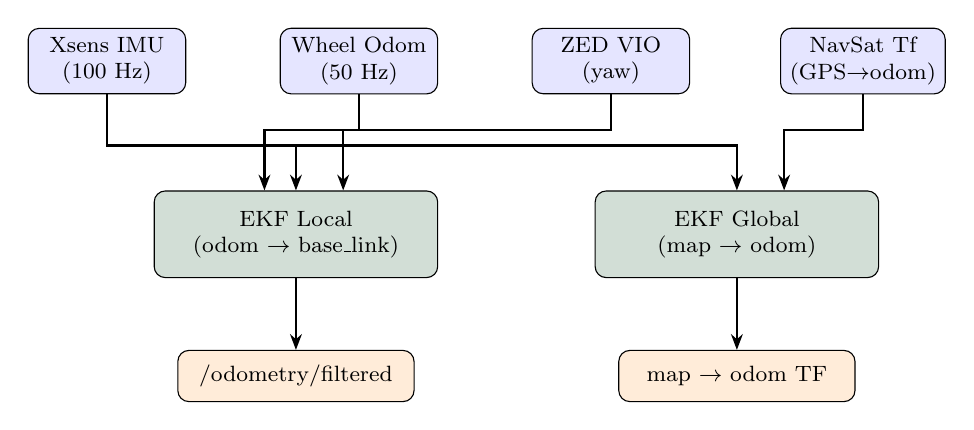
\begin{tikzpicture}[
        font=\footnotesize,
        ekf/.style={draw, rounded corners, fill=cppgreen!20, minimum width=3.6cm, minimum height=1.1cm, align=center},
        src/.style={draw, rounded corners, fill=blue!10, minimum width=2.0cm, minimum height=0.65cm, align=center},
        outnode/.style={draw, rounded corners, fill=orange!15, minimum width=3.0cm, minimum height=0.65cm, align=center},
        arr/.style={-{Stealth[length=2mm]}, thick},
    ]
        % Top row sources, spaced out evenly
        \node[src] (imu)    at (0,0)    {Xsens IMU\\(100 Hz)};
        \node[src] (wodom)  at (3.2,0)  {Wheel Odom\\(50 Hz)};
        \node[src] (zed)    at (6.4,0)  {ZED VIO\\(yaw)};
        \node[src] (navsat) at (9.6,0)  {NavSat Tf\\(GPS$\to$odom)};

        % Middle row: EKFs, each below its sources
        \node[ekf] (ekfL) at (2.4, -2.2) {EKF Local\\(odom $\to$ base\_link)};
        \node[ekf] (ekfG) at (8.0, -2.2) {EKF Global\\(map $\to$ odom)};

        % Bottom row: outputs
        \node[outnode] (oL) at (2.4, -4.0) {/odometry/filtered};
        \node[outnode] (oG) at (8.0, -4.0) {map $\to$ odom TF};

        % Arrows: sources to EKFs with clean down + sideways routing.
        % IMU feeds BOTH EKFs — draw as a small tee so it's visually obvious.
        \coordinate (imuTee) at ($(imu.south)+(0,-0.65)$);
        \draw[arr] (imu.south) -- (imuTee) -| (ekfL.north);
        \draw[arr] (imuTee) -| (ekfG.north);
        % Wheel odom -> local
        \draw[arr] (wodom.south) -- ++(0,-0.45) -| ([xshift=-0.4cm]ekfL.north);
        % ZED yaw -> local
        \draw[arr] (zed.south) -- ++(0,-0.45) -| ([xshift=0.6cm]ekfL.north);
        % NavSat (GPS) -> global
        \draw[arr] (navsat.south) -- ++(0,-0.45) -| ([xshift=0.6cm]ekfG.north);

        % EKFs -> outputs
        \draw[arr] (ekfL) -- (oL);
        \draw[arr] (ekfG) -- (oG);
    \end{tikzpicture}
    \caption{Dual-EKF sensor fusion. The local filter produces smooth odometry for the
    controller; the global filter anchors the local frame to GPS coordinates. ZED VIO is
    fused for yaw only to avoid lever-arm bias; GPS is fused in differential mode so noisy
    consumer-grade fixes integrate as deltas rather than creating costmap jumps.}
    \label{fig:ekf}
\end{figure}

The \textbf{local EKF} (\texttt{odom}~$\to$~\texttt{base\_link}) fuses three sources: the
Xsens IMU (roll, pitch, yaw, and angular velocities), wheel odometry from the actuator
node (linear velocity $v_x$ and yaw rate $\dot\psi$ from diff-drive forward kinematics, with
$v_y$ marked unobservable), and the ZED~X VIO yaw (differential, avoiding the lever-arm
bias). The \textbf{global EKF} (\texttt{map}~$\to$~\texttt{odom}) fuses the IMU stream
with GPS odometry from the \texttt{navsat\_transform\_node}, integrated in differential mode
with a 6$\sigma$ outlier-rejection threshold.

\subsection{Path Planning and Navigation}

The Nav2 stack provides path planning, trajectory generation, and behavior orchestration.
Key plugins and parameters for the Humble production build are listed in Table~\ref{tab:nav2}.

\begin{table}[H]
    \centering
    \small
    \caption{Nav2 Configuration (\texttt{nav2\_params\_humble.yaml})}
    \label{tab:nav2}
    \begin{tabularx}{\textwidth}{l X}
        \toprule
        \textbf{Component} & \textbf{Configuration} \\
        \midrule
        Planner & \texttt{nav2\_navfn\_planner::NavfnPlanner} (Dijkstra) --- chosen over SmacPlannerHybrid because the IGVC lane spacing (2--3~m) is narrower than the Hybrid planner's 2.31~m minimum turning radius \\
        Controller & \texttt{nav2\_mppi\_controller::MPPIController} --- DiffDrive motion model, 2000 rollouts, 56 timesteps, model $\Delta t$ 50~ms, 8 active critics \\
        Local costmap & 50$\times$50~m rolling, 0.2~m resolution; \texttt{stvl\_layer} + \texttt{semantic\_layer} (front/left/right) + \texttt{inflation\_layer} \\
        Global costmap & 100$\times$100~m rolling, 0.2~m resolution; \texttt{obstacle\_layer} (VLP-16) + \texttt{inflation\_layer} \\
        Footprint & Rectangular $1.00 \times 0.74$~m, $r_{\text{inscr}} = 0.5$~m \\
        Inflation & $r_{\text{infl}} = 0.65$~m, $k_{\text{scale}} = 3.0$ (smooth gradient for MPPI critic) \\
        Goal tolerance & $xy$ 2.0~m (IGVC waypoint acceptance), yaw 0.5~rad \\
        Controller frequency & 20~Hz; planner replans at 1~Hz via BT \texttt{RateController} \\
        \bottomrule
    \end{tabularx}
\end{table}

\textbf{Waypoint orchestration.} The \texttt{mission\_manager} node in \texttt{avros\_navigation}
loads the IGVC competition waypoints from \texttt{waypoints.yaml} as a lat/lon list, converts
each to the map frame via the \texttt{robot\_localization /fromLL} service, and fires
\texttt{NavigateToPose} action goals to Nav2 sequentially. The cursor advances when the
robot is within a 2.0~m acceptance radius (IGVC rule), and \texttt{ABORTED}/\texttt{CANCELED}
failures fall through to the next waypoint rather than halting the mission.

\textbf{Behavior tree.} The active BT (\texttt{navigate\_igvc\_autonav\_humble.xml}) wraps
the standard plan-follow pipeline with several IGVC-specific guards. An outer
\texttt{Timeout} of 45~s margins the 60~s hold-up-traffic disqualification rule. A
\texttt{RecoveryNode} retries the pipeline up to three times. Recovery actions form a
\texttt{RoundRobin} that escalates each attempt: clear costmap around robot $\to$ wait
2~s for stale semantic cells to decay $\to$ short backup (1.5~m at 0.08~m/s) $\to$ crawl
forward (0.15~m at 0.10~m/s). Spin-in-place is intentionally omitted: the
$1.00 \times 0.74$~m rectangular footprint sweeps a 2.48~m diameter circle when off-center,
exceeding the half-lane width and risking the IGVC 3-inch white-tape crossing penalty.

\subsection{Drive-by-Wire Control}
\label{sec:control}

The \texttt{actuator\_node} (Figure~\ref{fig:system_arch}, lower right) is the bridge from
Nav2 to the physical drivetrain. It subscribes to \texttt{/cmd\_vel} (from Nav2, teleop, or
the velocity smoother) and \texttt{/avros/actuator\_command} (from the webui for manual
override). Each control loop tick at 50~Hz:

\begin{enumerate}
    \item \textbf{Source arbitration.} A fresh \texttt{ActuatorCommand} takes priority over \texttt{cmd\_vel}; the source falls back to a hard zero if neither has been updated within \texttt{cmd\_timeout\_s} (0.5~s).
    \item \textbf{Slew-rate limit.} Linear: 0.5~m/s$^2$ accel / 1.5~m/s$^2$ brake. Angular: 1.0~rad/s$^2$. Protects the 12~V rail from motor inrush (which previously caused Jetson brown-outs) and gives smooth ride feel.
    \item \textbf{IMU-based assist.} When $|\omega_{\text{cmd}}| < 0.05$~rad/s, the current IMU yaw is locked and a P-controller ($K_p = 1.5$) drives the robot straight regardless of surface friction asymmetry --- ``heading hold.'' When $|\omega_{\text{cmd}}| \geq 0.05$~rad/s, the IMU yaw rate becomes feedback ($K_p = 0.3$) so a 0.5~rad/s command produces 0.5~rad/s on any surface --- ``gyro-stabilized turn.''
    \item \textbf{Diff-drive inverse.} $(v, \omega) \to (\text{L\_rpm}, \text{R\_rpm})$ using \texttt{track\_width\_m = 0.7366~m}, \texttt{m\_per\_motor\_rev = 0.01994~m}.
    \item \textbf{Serial write.} ASCII command \texttt{L<rpm> R<rpm>} is written over USB serial at 115200~baud to the Teensy 4.1.
\end{enumerate}

In parallel, the actuator node integrates wheel encoder feedback into a 50~Hz
\texttt{/wheel\_odom} \texttt{nav\_msgs/Odometry} message that the local EKF consumes.

\textbf{Firmware.} The Teensy 4.1 translates ASCII RPM commands into SparkMAX CAN velocity
setpoints at 1~Mbit/s and echoes encoder feedback at 50~Hz. Three independent timeouts
protect the drivetrain: a 300~ms serial watchdog on the Teensy, a 100~ms CAN heartbeat
timeout per SparkMAX, and a firmware clamp of $\pm$4600~RPM (1.53~m/s ground speed, below
the 5~mph IGVC cap).

\subsection{Simulation}

Development and regression testing use the \texttt{avros\_sim} package, which runs Webots
with a \texttt{cpp\_campus.wbt} world imported from the Cal Poly Pomona OpenStreetMap
extract. A custom Webots driver publishes simulated VLP-16, ZED, and GNSS topics that the
rest of the stack consumes unchanged, enabling perception and Nav2 development without
field time.

% ============================================================================
% 7. CYBER SECURITY
% ============================================================================
\section{Cyber Security Analysis}

\robotname{} follows the NIST Risk Management Framework (RMF) approach: identify threats
and impacted subsystems, classify by confidentiality / integrity / availability impact, and
apply NIST 800-53 controls.

\begin{table}[H]
    \centering
    \small
    \caption{Threat Model and Mitigations}
    \begin{tabularx}{\textwidth}{l X l}
        \toprule
        \textbf{Subsystem / Threat} & \textbf{Mitigation (NIST control)} & \textbf{C/I/A} \\
        \midrule
        Onboard network breach & Dedicated 192.168.13.0/24 subnet, WPA2 (SC-7) & L/H/H \\
        ROS~2 topic injection & CycloneDDS with DDS Security; network isolation (AC-3) & L/H/H \\
        WebSocket joystick hijack & HTTPS/WSS, fail-safe disconnect $\to$ E-stop (AC-3) & L/H/H \\
        GPS spoofing / multipath & Differential GPS fusion + 6$\sigma$ Mahalanobis rejection (SI-4, SI-7) & L/M/M \\
        SSH access to Jetson & Key-only authentication; password login disabled (AC-3, IA-2) & H/H/M \\
        Git repository tampering & Branch protection, PR review (CM-5) & M/H/L \\
        \bottomrule
    \end{tabularx}
\end{table}

\textbf{Defense in depth.} Safety-critical motion is gated by three independent stop
mechanisms: the physical E-stop button on the vehicle rear, the wireless E-stop relay held
by the judges during competition runs, and a software interlock in the actuator node that
zeroes \texttt{cmd\_vel} on stale input. Any one of the three removes power from the motors;
all three default to engaged on communication loss. Manual \texttt{ActuatorCommand} input
from the webui always takes priority over autonomous \texttt{cmd\_vel}, so a human operator
can override Nav2 at any time.

% ============================================================================
% 8. VEHICLE ANALYSIS
% ============================================================================
\section{Vehicle Analysis}
\label{sec:safety}

\subsection{Safety, Reliability, and Durability}

Safety is enforced at every layer: a hardware speed cap (4600~RPM $\to$ 1.53~m/s) in the
Teensy firmware, a 300~ms serial watchdog on the Teensy, a 100~ms CAN heartbeat timeout
per SparkMAX, a software slew-rate limit in the actuator node, and Nav2's MPPI collision
critic plus a costmap inflation radius of 0.65~m (inscribed radius plus margin). The MPPI
\texttt{CostCritic} uses \texttt{consider\_footprint: true} so the rectangular
$1.00 \times 0.74$~m footprint is swept along every rollout trajectory rather than only
the center point --- catching trajectories that would clip a thin painted lane line at
high steering angles.

\subsection{Failure Points and Resolutions}

\begin{table}[H]
    \centering
    \small
    \caption{Known Failure Modes and Mitigations}
    \begin{tabularx}{\textwidth}{l X X}
        \toprule
        \textbf{Layer} & \textbf{Failure} & \textbf{Mitigation} \\
        \midrule
        Mechanical & Fasteners loosen under vibration & Loctite + Nyloc nuts; periodic torque checks \\
        Electrical & Motor inrush brown-out on shared rail & Separate Jetson power rail \\
        Electrical & Wireless E-stop link loss & Heartbeat timeout cuts motor relay power \\
        Sensing & Encoder dropout & Local EKF reverts to IMU prediction \\
        Sensing & GPS multipath / dropout & 6$\sigma$ outlier rejection; differential fusion \\
        Perception & HSV threshold drift across lighting & Adaptive $V$-floor; live-tunable HSV bounds \\
        Costmap & Stale semantic cells linger & STVL 5~s decay; semantic raytrace clearing \\
        Software & Stale \texttt{cmd\_vel} & 300~ms watchdog forces motor stop \\
        \bottomrule
    \end{tabularx}
\end{table}

\subsection{Testing Methodology and Version Control}

Software is developed in a Git repository (\href{https://github.com/Paarseus/IGVC_ROS2}
{\texttt{github.com/Paarseus/IGVC\_ROS2}}) with feature branches, pull-request review, and
automated linting via \texttt{colcon test}. All parameters --- perception thresholds, EKF
covariances, Nav2 gains, MPPI critic weights, actuator slew limits --- live in
version-controlled YAML, so the system is reproducible from a clean checkout.

Testing progresses through four stages: bench (subsystem in isolation), simulation (Webots
full stack), low-speed field tests on a flat surface, and full-speed field tests on the
IGVC practice course.

% ============================================================================
% 9. UNIQUE AUTONAV AND SELF-DRIVE SOFTWARE
% ============================================================================
\section{Unique AutoNav and Self-Drive Software}

\robotname{} competes in both AutoNav and Self-Drive. The two challenges share most of the
software stack: HSV lane detection, LiDAR obstacle avoidance, dual-EKF localization, MPPI
control, and the actuator node are identical. The differences are in the orchestration layer.

\subsection{AutoNav-Specific Features}

\begin{itemize}
    \item \textbf{Lane following:} HSV white-lane mask from each of three ZED~X cameras feeds the local costmap's \texttt{semantic\_layer} as lethal cells; MPPI generates rollouts that stay inside the lane corridor.
    \item \textbf{Obstacle avoidance:} VLP-16 STVL marks barrels and signs in both costmaps; MPPI's \texttt{PreferForwardCritic} and \texttt{PathFollowCritic} bias rollouts toward forward motion along the global plan when no obstacles intrude.
    \item \textbf{Waypoint navigation:} \texttt{mission\_manager} converts lat/lon waypoints from \texttt{waypoints.yaml} into map-frame goals via the \texttt{/fromLL} service and fires sequential \texttt{NavigateToPose} actions with a 2~m acceptance radius (IGVC rule).
    \item \textbf{Ramp handling:} The 2D-mode EKF assumption holds for the IGVC ramp incline; pitch is monitored from the IMU. MPPI's cost-regulated velocity scaling automatically slows the robot near costmap inflation.
\end{itemize}

\subsection{Self-Drive-Specific Features}

\begin{itemize}
    \item \textbf{Teleoperation:} \texttt{avros\_webui} provides a phone-based proportional joystick via WebSocket; the same node is used for bench testing and Self-Drive demonstration runs.
    \item \textbf{E-Stop compliance:} Physical, wireless, and software E-stops are independently armed; the wireless relay is verified effective at $>$100~ft per IGVC qualification.
    \item \textbf{Speed governance:} Hardware-enforced 1.53~m/s ground-speed cap (3.4~mph, well under the 5~mph IGVC limit); software slew-rate limit ensures smooth starts and stops.
    \item \textbf{Heading stability:} The actuator node's IMU-based heading hold gives straight-line driving on uneven surfaces without operator correction.
\end{itemize}

% ============================================================================
% 10. PERFORMANCE ASSESSMENT
% ============================================================================
\section{Performance Assessment}

Table~\ref{tab:perf} summarizes the current readiness of each IGVC function as of report
submission. Detailed bench and field data are maintained in the \texttt{docs/} folder of
the repository.

\begin{table}[H]
    \centering
    \small
    \caption{IGVC Function Status}
    \label{tab:perf}
    \begin{tabularx}{\textwidth}{l X l}
        \toprule
        \textbf{Category} & \textbf{Function} & \textbf{Status} \\
        \midrule
        \multirow{4}{*}{Qualification} & Dimensions, E-stops, safety light & \placeholder{Complete} \\
        & Hardware-governed maximum speed & Complete \\
        & Lane following demonstration & \placeholder{Testing} \\
        & Obstacle avoidance demonstration & \placeholder{Testing} \\
        \midrule
        \multirow{3}{*}{AutoNav} & Autonomous control & \placeholder{Testing} \\
        & Waypoint navigation & \placeholder{Testing} \\
        & Ramp traversal & \placeholder{Not yet tested} \\
        \midrule
        \multirow{3}{*}{Self-Drive} & Teleoperation & Complete \\
        & Parking maneuvers & \placeholder{Not yet tested} \\
        & Lane changing & \placeholder{Not yet tested} \\
        \bottomrule
    \end{tabularx}
\end{table}

\begin{table}[H]
    \centering
    \small
    \caption{Measured Performance Targets}
    \begin{tabularx}{\textwidth}{X l l}
        \toprule
        \textbf{Parameter} & \textbf{Requirement} & \textbf{Measured} \\
        \midrule
        Maximum ground speed (hardware-governed) & $\le$5~mph & 3.4~mph (1.53~m/s) \\
        Wireless E-stop range & $\ge$100~ft & \placeholder{measured~ft} \\
        Obstacle detection range (VLP-16, local costmap) & $\ge$2~m & 15~m \\
        Obstacle detection range (VLP-16, global costmap) & $\ge$2~m & 50~m \\
        Battery runtime & $\ge$5~min & \placeholder{measured~min} \\
        Course completion (Webots sim) & $\le$6~min & \placeholder{measured~min} \\
        \bottomrule
    \end{tabularx}
\end{table}

\placeholder{Add a short paragraph summarizing current readiness, strengths, and the
remaining work plan in the final weeks before competition.}

% ============================================================================
% REFERENCES
% ============================================================================
\section*{References}
\addcontentsline{toc}{section}{References}

\begin{enumerate}[leftmargin=*]
    \item S.~Macenski, F.~Mart{\'\i}n, R.~White, J.~Gin{\'e}s Clavero, ``The Marathon~2: A Navigation System,'' \textit{IEEE/RSJ IROS}, 2020. (Nav2)
    \item S.~Macenski et al., ``On Use of Nav2 MPPI Controller,'' ROSCon, 2023.
    \item T.~Moore and D.~Stouch, ``A Generalized Extended Kalman Filter Implementation for the Robot Operating System,'' \textit{Advances in Intelligent Systems and Computing}, 2016. (\texttt{robot\_localization})
    \item S.~Macenski, ``\texttt{spatio\_temporal\_voxel\_layer},'' GitHub, 2019--present.
    \item Kiwi Campus, ``\texttt{semantic\_segmentation\_layer} Nav2 plugin,'' GitHub, 2023--present.
    \item Sooner Competitive Robotics, ``IGVC 2025 Design Report: Twistopher,'' University of Oklahoma, 2025. \url{http://www.igvc.org/design/2025/7.pdf}
    \item Ville Robotics, ``IGVC 2024 Design Report: ALiEN 5.0,'' Millersville University, 2024. \url{http://www.igvc.org/design/2024/8.pdf}
    \item REV Robotics, ``SPARK MAX Documentation,'' 2024. \url{https://docs.revrobotics.com/brushless/spark-max/overview}
    \item PJRC, ``Teensy 4.1 Development Board.'' \url{https://www.pjrc.com/store/teensy41.html}
    \item Stereolabs, ``ZED~X and ZED SDK Documentation.'' \url{https://www.stereolabs.com/docs}
    \item Xsens / Movella, ``MTi-680G Product Documentation.'' \url{https://www.movella.com/products/sensor-modules/xsens-mti-680g}
    \item Velodyne Lidar, ``VLP-16 User Manual,'' 2023.
    \item IGVC Rules Committee, ``33rd Annual IGVC Official Competition Details, Rules, and Format,'' 2026. \url{http://www.igvc.org/}
\end{enumerate}

\end{document}
